\section{Lösung und Konzepte}\label{sec:02_03_loesung_konzept}
\subsection{Standard Aufbau eines Crawlers}
\begin{wrapfigure}{R}{0.4\textwidth}
  \centering
    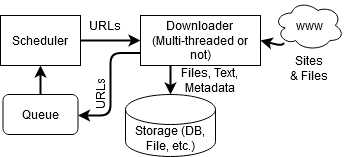
\includegraphics[width=0.4\textwidth]{images/02-Crawler/Crawler-Standard-Crawler.png}
  \caption{\label{fig:standardCrawler}Crawler: Standard Aufbau}
\end{wrapfigure}
Ein Crawler besteht in der Regel aus zwei wichtigen Teilen: ein Downloader und ein Scheduler. Der Downloader ist mit dem Webserver verbunden und lädt die Webseite(n) sowie alle erwünschten Dateien herunter. Der Scheduler ist, wie der Name schon sagt, für die Planung zuständig und erteilt dem Downloader URLs nach internen Priorisierung-Mechanismen (als Liste FIFO und als Graph mit DFS und BFS ~\cite{ThomasAlgorithms2009}--\cite{DonaldKnuth1998}). 
\subsection{Crawler Mechanismus}
Für unseren speziellen Fall, wird die Aufgaben von dem Scheduler vom Crawl-Manager übernommen, der sowohl für die Planung als auch für die Steuerung (Start, Pause, Stopp, Zustand) laufender Crawl-Aufgaben zuständig ist. Der Crawl-Manager erzeugt für jede URL ein Thread (Page-Crawler), dessen Aufgabe darin besteht die Seite herunterzuladen, mit seinem Page-Analyser nach relevanten Inhalten in der Seite zu suchen (URLs, Dateien, Action-Links: Javascript, etc.) und bei Bedarf weitere parallele Sub-Threads für den Download, das Parsen und die Speicherung der relevanten Dateiinhalte (Protokollen, Stammdaten, weitere Metadaten). Dieser Mechanismus wird durch die Abb.~\ref{fig:funktionsprinzipCrawler} und die Abb.~\ref{fig:crawlEinerUrl} veranschaulicht.

\begin{figure}[H]
    \centering
    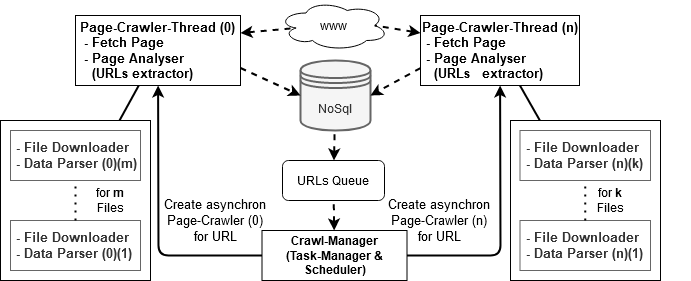
\includegraphics[width=5in]{images/02-Crawler/Crawler-Process-Diagram (Multithreading).png}
    \caption{Funktionsprinzip des unseres Crawlers}
    \label{fig:funktionsprinzipCrawler}
\end{figure}

\begin{figure}[H]
    \centering
    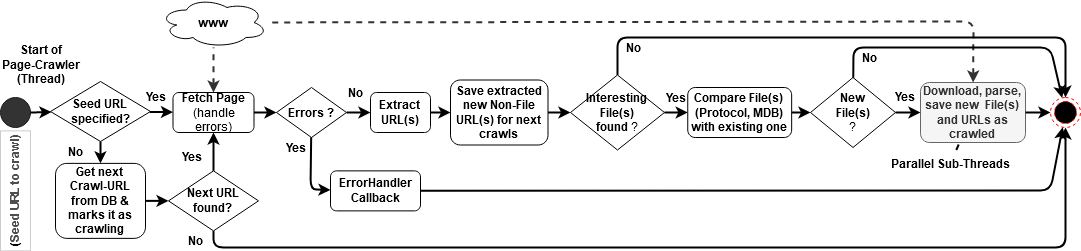
\includegraphics[width=5.5in]{images/02-Crawler/Crawler-Process-Diagram (Page-Crawler).png}
    \caption{Page-Crawler für eine URL}
    \label{fig:crawlEinerUrl}
\end{figure}
\noindent
Ein Crawl auf einer Seite (durch den Page-Crawl) kann in einer durch den Scheduler (Crawl-Manager) regelmäßig gemacht werden, in dem dieser nach einer bestimmten Zeit einen neuen Page-Crawl-Thread startet. Die Frequenz der Generierung dieses Threads orientiert sich an dem Sitzungskalender des Bundestags~\cite{Sitzungskalender2021}. Dieser Kalender sieht vor, dass Sitzungen an bestimmten Wochentagen zwei bis vier Wochen pro Monat (abgesehen von August: Ferien) stattfinden. Darauf basierend ist die Entscheidung getroffen worden, die Frequenz auf einmal pro Tag von Montag bis Freitag (mit der Möglichkeit bei Bedarf den Crawler in der Ferienzeit zu stoppen) festzulegen. So lässt sich eine Sperrung wegen zu häufiger Abfragen verhindern. Bei Manchen Server (durch Regeln oder Server-Admin) kann aber ein sich wiederholender Abfrage-Muster (wie eine Abfrage jeden Tag um dieselbe Uhrzeit) auch zu einer Sperrung der IP (Rechner) führen. Aus diesem Grund wird zusätzlich zur Frequenz ein Zufallsfaktor verwendet. Ein Page-Crawl-Thread wird zwar von Montag bis Freitag um 23Uhr durch den Crawl-Manager gestartet, allerdings wartet dieser Thread ein zufällige Zeit $t$ (mit $10 \leq t \leq 7200 $) bis er den tatsächlichen Crawl durchführt. Während und nach dem Crawl-Prozess werden Daten (und Dateien) manipuliert, analysiert und gespeichert. Diese Vorgänge sowie die dafür verwendeten Datenstrukturen werden im nächsten Abschnitt beleuchtet. 

\subsection{Daten-Parser und Database-Modell}
- Parser für die 19. Legislaturperiode\\
- Parser für die 18. Legislaturperiode\\
- ER-Diagramm und Beschreibung des DB-Modells

\subsection{Gesamter Aufbau der Lösung}
Die gesamte Lösung besteht aus vier Komponenten und einer Datenbank, wie auf die Abb.~\ref{fig:crawlerKompoenenten} dargestellt. 
\begin{itemize}
    \item \textbf{Crawl-Manager}: Taskmanager und Scheduler
    \item \textbf{Crawl-Utilities}: Liefert die für den Crawl-Prozess nötigen Funktionalitäten (Page-Fetcher, Page-Analyser, Downloader, Data-Parser)
    \item \textbf{DB-Manager}: Verwaltet den Zugriff auf die Datenbank 
    \item \textbf{Rest-ServiceProvider}: Rest-API für die Steuerung des Crawl-Manager und den eingeschränkten Zugriff auf die DB-Daten
    \item \textbf{Datenbank}: NoSql (MongoDB) Datenbank für die Sicherung der Daten
\end{itemize}

\begin{figure}[H]
    \centering
    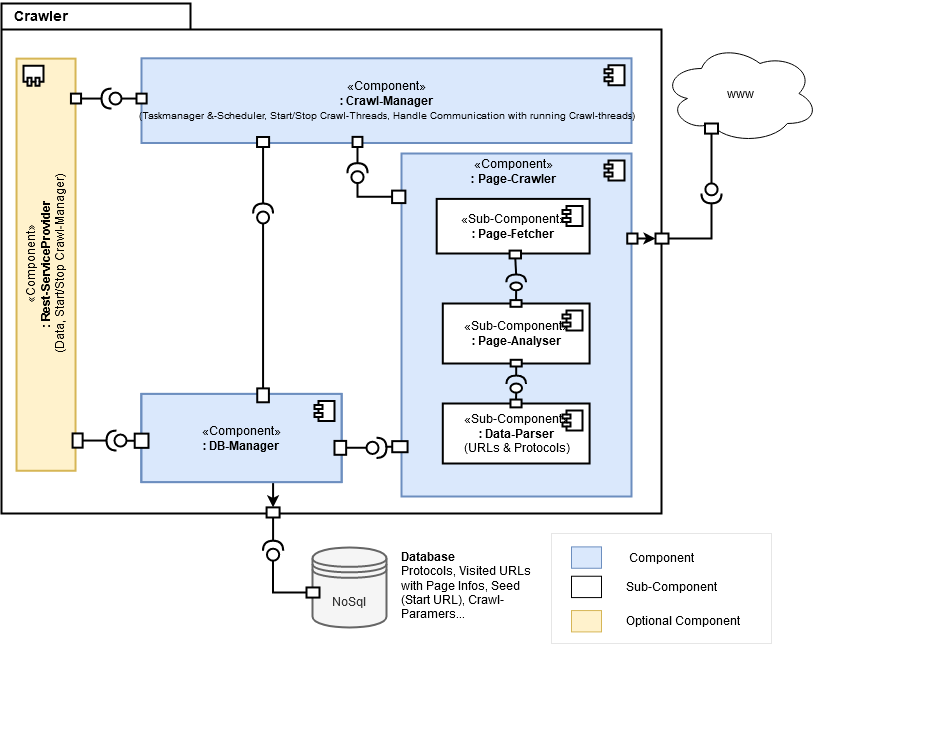
\includegraphics[width=5in]{images/02-Crawler/Crawler-Component-Diagram.png}
    \caption{Crawler: Komponentendiagramm}
    \label{fig:crawlerKompoenenten}
\end{figure}
\noindent
Am Ende eines Crawl-Prozess, bei dem neue Protokolle oder Stammdaten geladen worden sind, wird die Gruppe-Kommunikationsmodell die Liste aller Protokollen sowie Stammdaten über deren Rest-API~\cite{Cme2021} als Json-Datei mitgeteilt. Die Gruppe-Kommunikationsmodell kann dann asynchron die entsprechenden Dateien aus unseren Datenbank holen.